% Final
\section{Návrh architektury aplikace}

% Final
Při návrhu architektury jsem se rozhodl vycházet z architektury původní aplikace. Systém je rozdělen do frontendové a backendové části. Komunikace mezi těmito částmi probíhá prostřednictvím REST API. Dále je v systému zavedený mock API, který simuluje chování REST API a umožňuje tak frontendovou část aplikace testovat a vyvíjet nezávisle na backendové části. Tento přístup jsem se rozhodl zachovat, protože zjednodušuje paralelní vývoj obou částí a umožňuje průběžně testovat chování frontendové části aplikace nezávisle na stavu backendové části. Architektuře backendové části aplikace včetně návrhu API se věnuje kolega Bc. Jakub Vondráček v rámci své diplomové práce.

% Final
Frontendová část je tvořena webovou aplikací postavenou na frameworku Next.js. Oproti původní aplikaci jsem se rozhodl do systému zavést oddělené knihovny komponentů \texttt{@eduriam/ui-core} a \texttt{@eduriam/ui-x}. Knihovna \texttt{@eduriam/ui-core} bude obsahovat základní komponenty uživatelského rozhraní, zatímco knihovna \texttt{@eduriam/ui-x} bude obsahovat komplexnější komponenty využívané zejména ve výukových částech aplikace. Cílem tohoto rozdělení je oddělit obecně použitelné UI komponenty od aplikační logiky a umožnit tak jejich opětovné využití v různých částech projektu.

% Final
Kromě těchto hlavních částí dále existuje webová stránka aplikace a systém pro správu obsahu aplikace. Tyto části systému nejsou součástí této práce, nicméně budou využívat zmíněné knihovny komponentů, a je tak nutné tyto části zohlednit při návrhu architektury. Přehled architektury aplikace z pohledu frontendu je znázorněn na obrázku \ref{fig:architecture}.

% Final
\begin{figure}[!h]
    \centering
    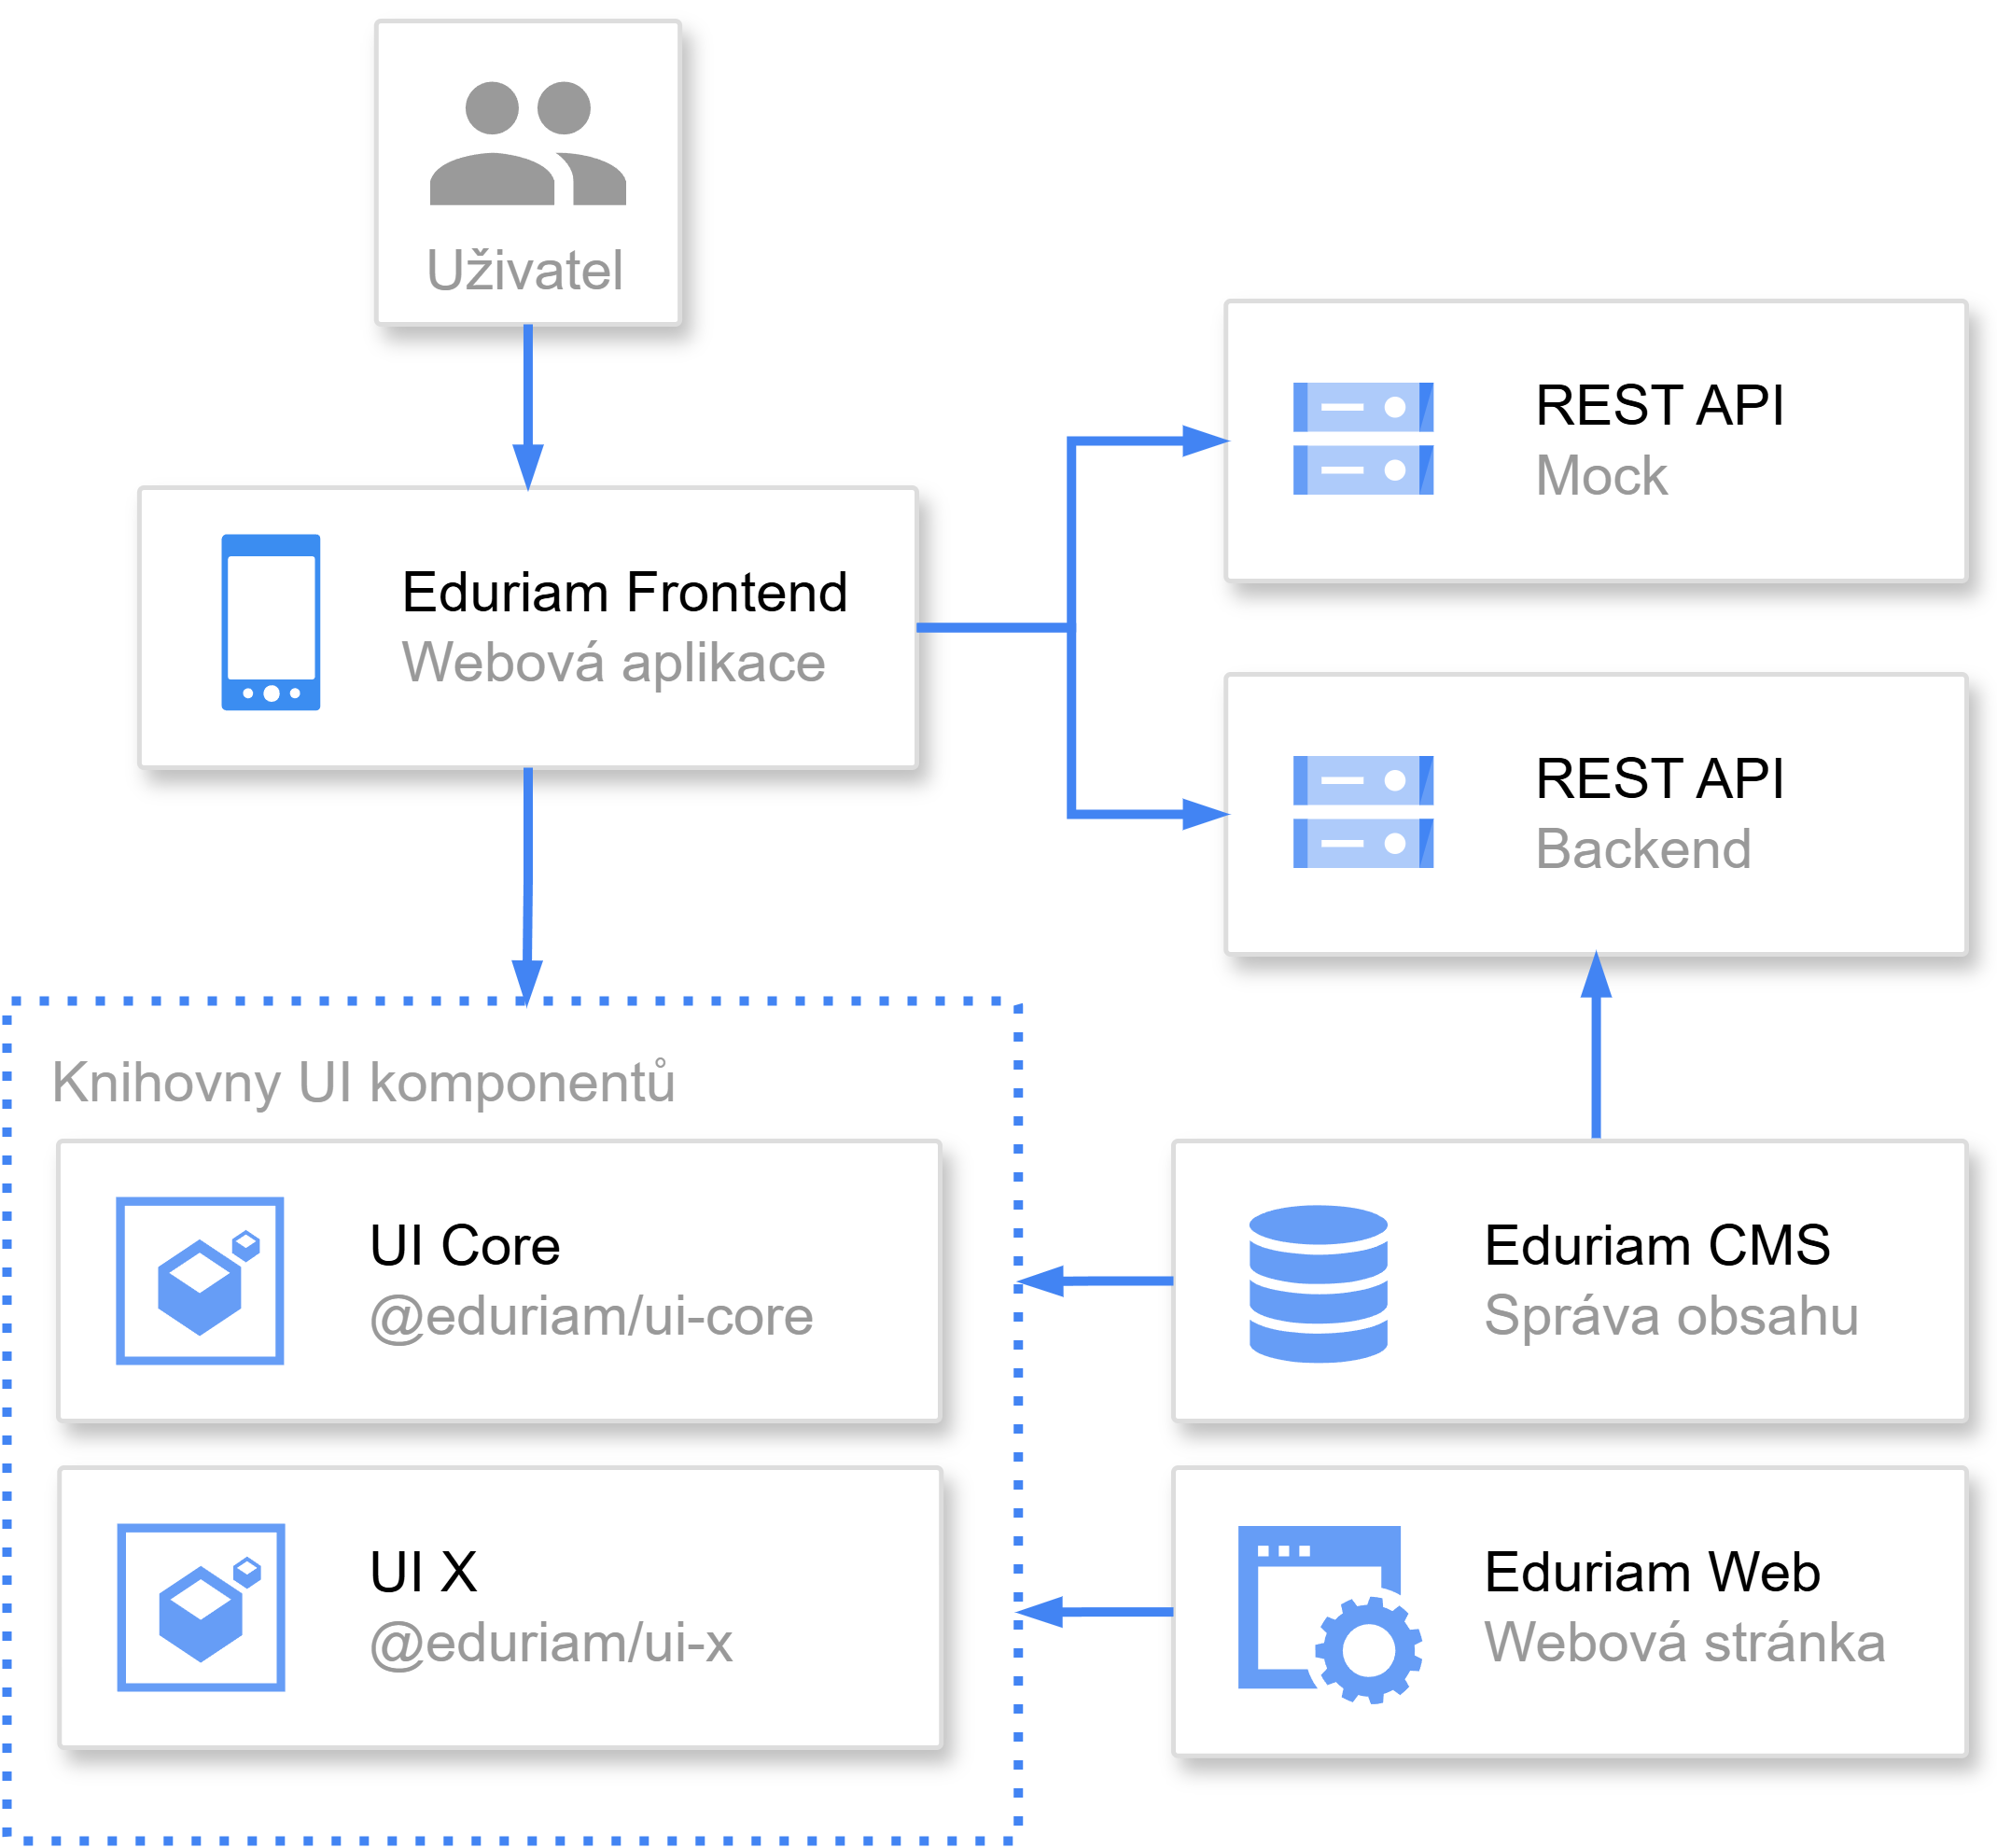
\includegraphics[width=\textwidth]{./images/diagrams/architecture.png}
    \caption{Základní návrh architektury aplikace}
    \label{fig:architecture}
\end{figure}
